\chapter{Results and Discussion}\label{results}

\section{Results and Discussion}

\subsection{Experiment-1: Model performance on a small corpous}

\paragraph{Word2Vec-ESN Model:}


\paragraph{Model Variant-2:} The model Variant-2, on the other hand, with a reservoir of size 600 neurons, produced the classification scores [write score here] during cross-validation. 

\subsection{Experiment-2: Generalization Capabilities} \label{exp-2}

\paragraph{Word2Vec-ESN model:} When the model was initially trained and tested the model on all the 462 sentences. The model learned the full corpus-462 with $0.55\%$ meaning error and $1.64\%$ sentence error in SCL mode and $0.16\%$ meaning error and $0.52\%$ sentence error in SFL mode. Using the 10-fold cross validation, the model generalized to $8.68\% (\pm 1.01\%) $ meaning error and $24.09\% (\pm 2.38\%)$ sentence error in SCL mode. Whereas in the SFL mode the optimal meaning and sentence error were observed as $8.88\% (\pm 0.14\%)$ and $25.17\% (\pm 0.01\%)$ respectively.

We compared the performance of Word2Vec-ESN model with $\theta RARes$ model which takes the sentences in grammatical form and words are represented in localist fashion. As illustrated in Table \ref{tab:corpus-462_errors}, one can see that $\theta RARes$ model, in SFL mode,  learned all the constructions thouroughly during training whereas the Word2Vec-ESN model learned with small errors. During testing, we can see an improvement of $8.04 \%$ sentence error in SCL mode with Word2Vec-ESN langugae model, whereas the meaning error dropped by $1.25 \%$. However, considering the standard deviation, we can also say that the meaning error remained almost equivalent in both the Word2Vec-ESN and $\theta RARes$ model. In SFL mode, both the meaning and sentence errors remained nearly same in both the models. It can also be observed that with Word2Vec-ESN model, the performance of the model is improved mainly in SCL mode as compared to SFL mode, whereas it was vice-versa in $\theta RARes$ model. 

%NOTE: 08/09/2016 results are copied after the simulation and are final, no need to change.
\begin{table}
\centering
\begin{threeparttable}
\caption{Mean and standard deviation of meaning and sentence error on train and test set of coprus-462 in different learning modes.}
\label{tab:corpus-462_errors}
\rowcolors{2}{white}{gray!25}
\begin{tabular}{llrrrrrrrr}
  \toprule
  \hiderowcolors   
  &  & \multicolumn{4}{c}{Word2Vec-ESN} & \multicolumn{4}{c}{$\theta RARes$} \\
  \cmidrule(lr){3-6}   \cmidrule(lr){7-10}
  
  &  & \multicolumn{2}{c}{Corpus 462} & \multicolumn{2}{c}{462 scrambled} & \multicolumn{2}{c}{Corpus-462} & \multicolumn{2}{c}{462 scrambled} \\
  \cmidrule(lr){3-4} \cmidrule(lr){5-6}  \cmidrule(lr){7-8} \cmidrule(lr){9-10}  
  
  
   						& 		& ME 	& SE 		& ME 	 & SE 		& ME 	& SE		& ME 	& SE 		\\
  \midrule
  \showrowcolors
  \textbf{SCL\ train} 	& mean 	& 0.55 & 1.64  		& 6.68  & 26.80	 	& 0.12 & 1.21 	& 4.81  & 20.43	\\
   			    		& std 	& 0.06 & 0.12 		& 0.67  & 1.64 		& 0.03 & 0.30 	& 0.30  & 1.25	\\
   			    		
  \textbf{SCL\ test} 	& mean  & 8.68 & 24.09 		& 70.15 & 99.26 	& 7.43 & 32.13 	& 74.15 & 99.89	\\
  			   			& std  	& 1.01 & 2.38 		& 1.24  & 0.29  	& 0.52 & 1.35 	& 0.80  & 0.15	\\
  			   			
  \textbf{SFL\ train} 	& mean 	& 0.16 & 0.52 		& 9.38  & 35.58 	& 0.00 & 0.00 	& 0.00  & 0.00	\\
  				 		& std 	& 0.09 & 0.25 		& 0.69  & 3.40 		& 0.00 & 0.00 	& 0.00  & 0.00	\\
  				 		
  \textbf{SFL\ test}	& mean  & 8.88 & 25.17 		& 67.87 & 99.26 	& 9.18 & 24.37 	& 73.39 & 99.91	\\
  			  			& std 	& 0.14 & 0.01		& 0.10  & 0.33  	& 0.57 & 1.19 	& 0.96  & 0.11	\\
  \bottomrule
\end{tabular}
\begin{tablenotes}
\small
\item 
Meaning (ME) and Sentence error (SE) in different learning modes with Word2Vec-ESN model using distributed word embeddings and $\theta RARes$ model \cite{xavier:2013:RT} which uses grammatical form and localist representation of words of sentences. The errors are given in percentage with 2 decimal precision. SCL: Sentence Continuous Learning; SFL: Sentence Final Learning; std: standard deviations. Simulations were done with 5 model instances with reservoir of 1000 neurons.
\end{tablenotes}
\end{threeparttable}
\end{table}

\paragraph{Word2Vec-ESN model variant:} 

Table \ref{tab:corpus-462-scores}, illustrates the training and cross-validation classification scores of simulations performed with the model variant in both the configurations as described in Experiment-2 (see section \ref{exp-2}). The word2vec-ESN model variant, in configuration-1, when trained and tested on all 462 sentences of corpus-462, the model learned to label the argument-predicate pairs in the sentences with Precision (Pr), Recall (Re) and F1-Score (F1) of $97.46 \%$, $92.29 \%$, $94.65 \%$ respectively. When tested using 10-fold cross validation for generalization, the model genralized with Pr = $96.76 \% (\pm 0.08 \%)$, Re = $91.78 \% (\pm 0.08 \%)$ and F1 = $93.99 \%(\pm 0.09 \%)$. Notice the marginal difference between the training and cross validation scores, indicating that the model variant in configuration-1 is generalizing well on untrained sentences and is not overfitting.

When using the sentences transformed to GF and localist word representations as an input to ESN (configuration-2), the model variant learned the sentences with Pr = $61.96 \% (\pm 0.07\%)$, Re = $67.69 \% (\pm 0.29\%)$, F1 = $63.55 \% (\pm 0.17\%)$ during training. With 10-fold cross-validation the model generalized with Pr = $61.91 \% (\pm 0.07\%)$, Re = $68.20 \% (\pm 0.46\%)$ and F1 = $63.71 \% (\pm 0.22\%)$. It can be noticed that the model variant in this configuration was not able to learn the thematic role during training and hence not able to generalize during testing.

\begin{table}
\centering
\begin{threeparttable}
\caption{Classification scores produced by Word2Vec-ESN model variant on corpus-462 in two configurations.}
\label{tab:corpus-462-scores}
\rowcolors{2}{white}{gray!25}
\begin{tabular}{llll}
  \toprule
  \hiderowcolors   
  &  & \multicolumn{1}{c}{Configuration-1} & \multicolumn{1}{c}{Configuration-2} \\
   			
  \midrule
  \showrowcolors
  \textbf{Precision} 	& test 		& 96.76 ($\pm$ 0.08) 	 	& 61.91 ($\pm$ 0.07) 	\\
   			    	  	& train 	& 97.46 ($\pm$ 0) 			& 61.96 ($\pm$ 0.07) 	\\
   			    		
  \textbf{Recall} 		& test  	& 91.78 ($\pm$ 0.08) 	 	& 68.20 ($\pm$ 0.46)  	\\
  			   			& train 	& 92.29 ($\pm$ 0.22) 		& 67.69 ($\pm$ 0.29)	\\
  			   			
  \textbf{F1-Score} 	& test 		& 93.99 ($\pm$ 0.09)	 	& 63.71 ($\pm$ 0.22) 	\\
  				 		& train 	& 94.65 ($\pm$ 0)		 	& 63.55 ($\pm$ 0.17)		\\  				 		
  
  \bottomrule
\end{tabular}
\begin{tablenotes}
\small
\item 
Classification scores (in  $\%$) of Word2Vec-ESN model variant during training and testing condition. Configuration-1: word2vec word vectors are input to ESN. Configuration-2: Sentences transformed to grammatical form and localist word vectors are input to ESN. Simulations were done with 5 instance of model variant with reservoir of 1000 neurons.
\end{tablenotes}
\end{threeparttable}
\end{table}

% CONFUSION MATRIX
\begin{figure}[hbtp]
\centering
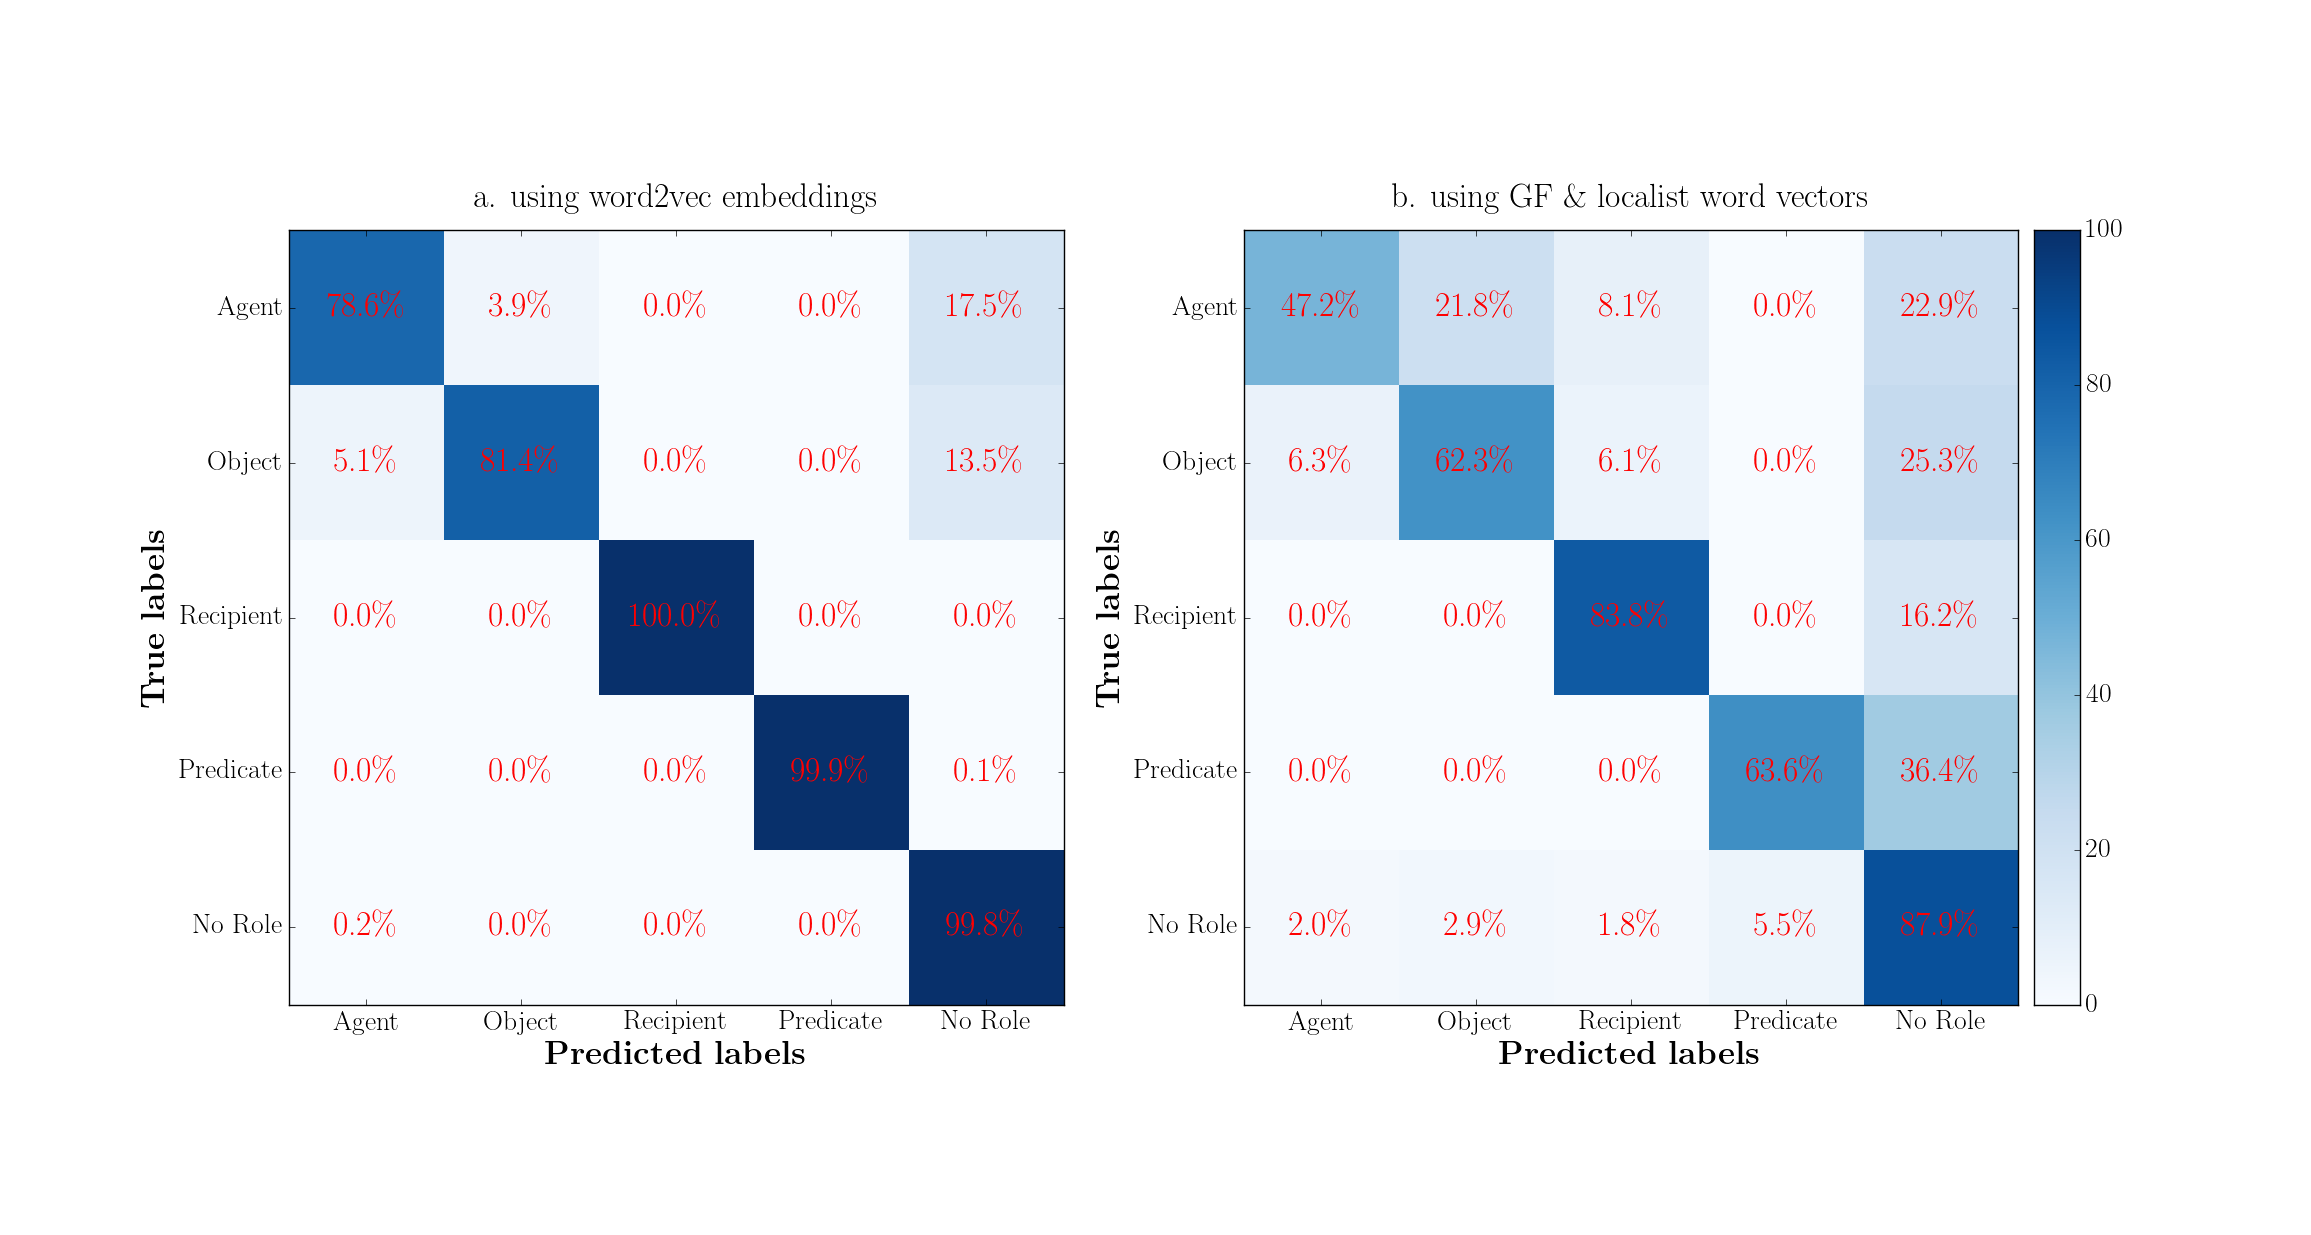
\includegraphics[width=1.0\linewidth]{confusion_matrix}
\caption[Normalized confusion matrix on corpus 462 with Word2Vec-ESN model variant] {\textbf{Normalized confusion matrix with Word2Vec-ESN model variant:} The confusion matrix with true roles (in rows) and predicted roles (in columns). The top-left to bottom-right diagonal shows the percentage of words whose roles are predicted correctly. Everything other than this diagonal represents the incorrect prediction of roles. Model identified almost all words labelled as Recipient , Predicate and No Role and made some errors in predicting role Agent and Object. The results were obtained with reservoir of 1000 neurons and 10 fold-cross validation.}
\label{fig:confusion_matrix}
\end{figure}

Figure \ref{fig:confusion_matrix} shows the confusion matrix, plotted using cross-validation results of the model variant in configuration-1 and configuration-2 (See section \ref{exp-2}). The corresponding classification scores of individual roles produced by model variant during 10-fold cross-validation in both the configuration are also reported in Table\ref{tab:classsification-scores-21}.

As seen in confusion matrix (see fig. \ref{fig:confusion_matrix}), when using word2vec word vectors as an input to ESN, the model predicted the words with role `Recipient', `Predicate' and `No Roles' almost without making any errors. The model predicted $78.6 \%$ of the words with role `Agent' correctly, whereas $3.9 \%$ and $17.5 \%$ of the words with role `Agent' were incorrectly predicted as `Object' and `No Role' respectively. Similarly, $81.4 \%$ of the words with role `Object' were correctly classified, whereas $ 5.1 \%$ of the words with actual roles as `Object' were misclassifed as `Agent' and $13.5 \%$ as `No Role'. On the other hand, only $0.2 \%$ the words with actual role `No Role' were wrongly predicted as 'Agent'. 

Using the sentences in GF along with localist word vectors, as an input to ESN, the roles `Recipient' and `No Role' were correcly predicted with least errors of $16.2 \%$ and $12.1 \%$. The model variant wrongly predicted all the roles as `No Role', where the `Predicate' being the highest role to be misclassified as 'No Role' ($36.4 \%$). The model seems to be confused between the role `Agent' and 'Object', where $21.8 \%$ of words with roles `Agent' were incorrectly predicted as `Object', whereas $6.3 \%$ of words with actual role as `Object' were misclassified as `Agent'. Also, the words with roles `Agent' and `Object' were confused with the role `Recipient', where $8.1 \%$ of words with the role `Agent' were wrongly predicted as `Recipient' and $6.1 \%$ of the words with role `Object' were incorrectly predicted as 'Recipient'. 

While comparing the predictions made by the model variant in both the configurations, it was observed that the roles `Agent' and `Object' made most of error in predictions as compared to other roles. When using GF sentence form and localist word vectors, the roles `Agent' and `Object' were wrongly predicted as 'Recipient', whereas while using word2vec vectors the model, this misprediction do not exist. Comparing the false predictions made by model variant in both the configurations, it was also observed that in configuration-1 (while using word2vec word vectors), the incorrect prediction were comparatively less. In configuration-1, all the words with roles `Recipient', `Predicate' and `No Role' were predicted almost without any errors whereas in configuration-2, the model variant misclassified these roles respectively by $16.2 \%$, $36.4\%$, and $12.1 \%$.


%NOTE: 08/09/2016 results are copied after the simulation and are final, no need to change.
\begin{table}[h]
\centering
\begin{threeparttable}
\caption{Training and testing classification scores for individual roles when using Word2Vec-ESN model variant in two different configurations.}
\label{tab:classsification-scores-21}
\rowcolors{2}{gray!25}{white}
\begin{tabularx}{\textwidth}{@{}llYYYYYYY@{}}
\hiderowcolors
\toprule
  &  & \multicolumn{3}{c}{Configuration-1} & \multicolumn{3}{c}{Configuration-2}& \\  
\cmidrule(lr){3-5}   \cmidrule(lr){6-8}
   
Role 				& 			& Pr   & Re  & F1 		& Pr  &  Re & F1 		&  Support  \\
\showrowcolors
\midrule
               
\textbf{Agent}		&test 		& 0.92 & 0.79 & 0.85 	& 0.63 & 0.47 & 0.54	& 888  \\
					&train  	& 0.94 & 0.80 & 0.86 	& 0.64 & 0.46 & 0.53	& 892  \\
\textbf{Object}		&test 		& 0.95 & 0.81 & 0.88 	& 0.51 & 0.62 & 0.56	& 791  \\
					&train  	& 0.96 & 0.82 & 0.88 	& 0.51 & 0.61 & 0.56	& 794  \\
\textbf{Recipient}	&test 		& 1.00 & 1.00 & 1.00 	& 0.52 & 0.84 & 0.64	& 382  \\
					&train  	& 1.00 & 1.00 & 1.00 	& 0.52 & 0.83 & 0.64	& 384  \\
\textbf{Predicate}	&test		& 1.00 & 1.00 & 1.00 	& 0.51 & 0.64 & 0.57	& 888  \\
					&train  	& 1.00 & 1.00 & 1.00 	& 0.51 & 0.64 & 0.57	& 892   \\
\textbf{No Role}	&test 		& 0.97 & 1.00 & 0.99 	& 0.92 & 0.88 & 0.90	& 9776  \\
					&train  	& 0.97 & 1.00 & 0.99 	& 0.91 & 0.88 & 0.90	& 9823  \\
\bottomrule
\end{tabularx}
\begin{tablenotes}
\small
\item Training and cross-validation classification scores (precision upto 2 decimals) for each output roles predicted by the model variant in two configuration. Support for each role: actual number of instances, is also shown in last column. Simulation condition: 1000 reservoir neurons, 10-fold cross-validation.
\end{tablenotes}
\end{threeparttable}
\end{table}

\subsection{Experiment-3: Effect of Corpus structure} 

\paragraph{Word2Vec-ESN model: } As illustrated in table \ref{tab:corpus-462_errors}, it was observed that when using the scrambled corpus as an input to the Word2Vec-ESN model, the model learned with low error rates of $ME = 6.68 \%$ and $SE = 26.80 \%$ in SCL mode, but while testing, the model generalized with cross-validation error rates of $ME = 70.15 \% $ and $SE = 99.26 \%$. Similarly, in SFL mode the model learned with low error rates of $ME = 9.38 \%$ and $SE = 35.58 \%$  but during cross-validation high error rates of $ME = 67.87 \%$ and $SE = 99.26 \% $ was observed. Notice that the model learned the scrambled corpus with low error rates while training but during the cross-validation resulted into high error rates.

\subsection{Experiment-4: Effect of Reservoir size}

\paragraph{Word2Vec-ESN model: } Figure \ref{fig:reservoir_size_1} shows the effect of reservoir size on the cross-validation errors rates (i.e. meaning and sentence error). The meaning and sentence error continuously drops with increase in reservoir size from 90 to 1098 in both the learning modes. The meaning error in SFL mode slightly increases ($\approx 1\%$), whereas it remains unchanged in SCL mode as the reservoir size is further increased from size 1098. On the other hand, the sentence error in SFL mode slightly increases whereas in SCL mode it is negligibally dropped when the reservoir size is further increased from 1776 to 2882 and remains stable after that. Overall, it was observed that both the meaning and sentence cross-validation error rates reduces with increase in reservoir size but asymptotes when the reservoir size is above 1000 on corpus-462.

\begin{figure}[hbtp]
\centering
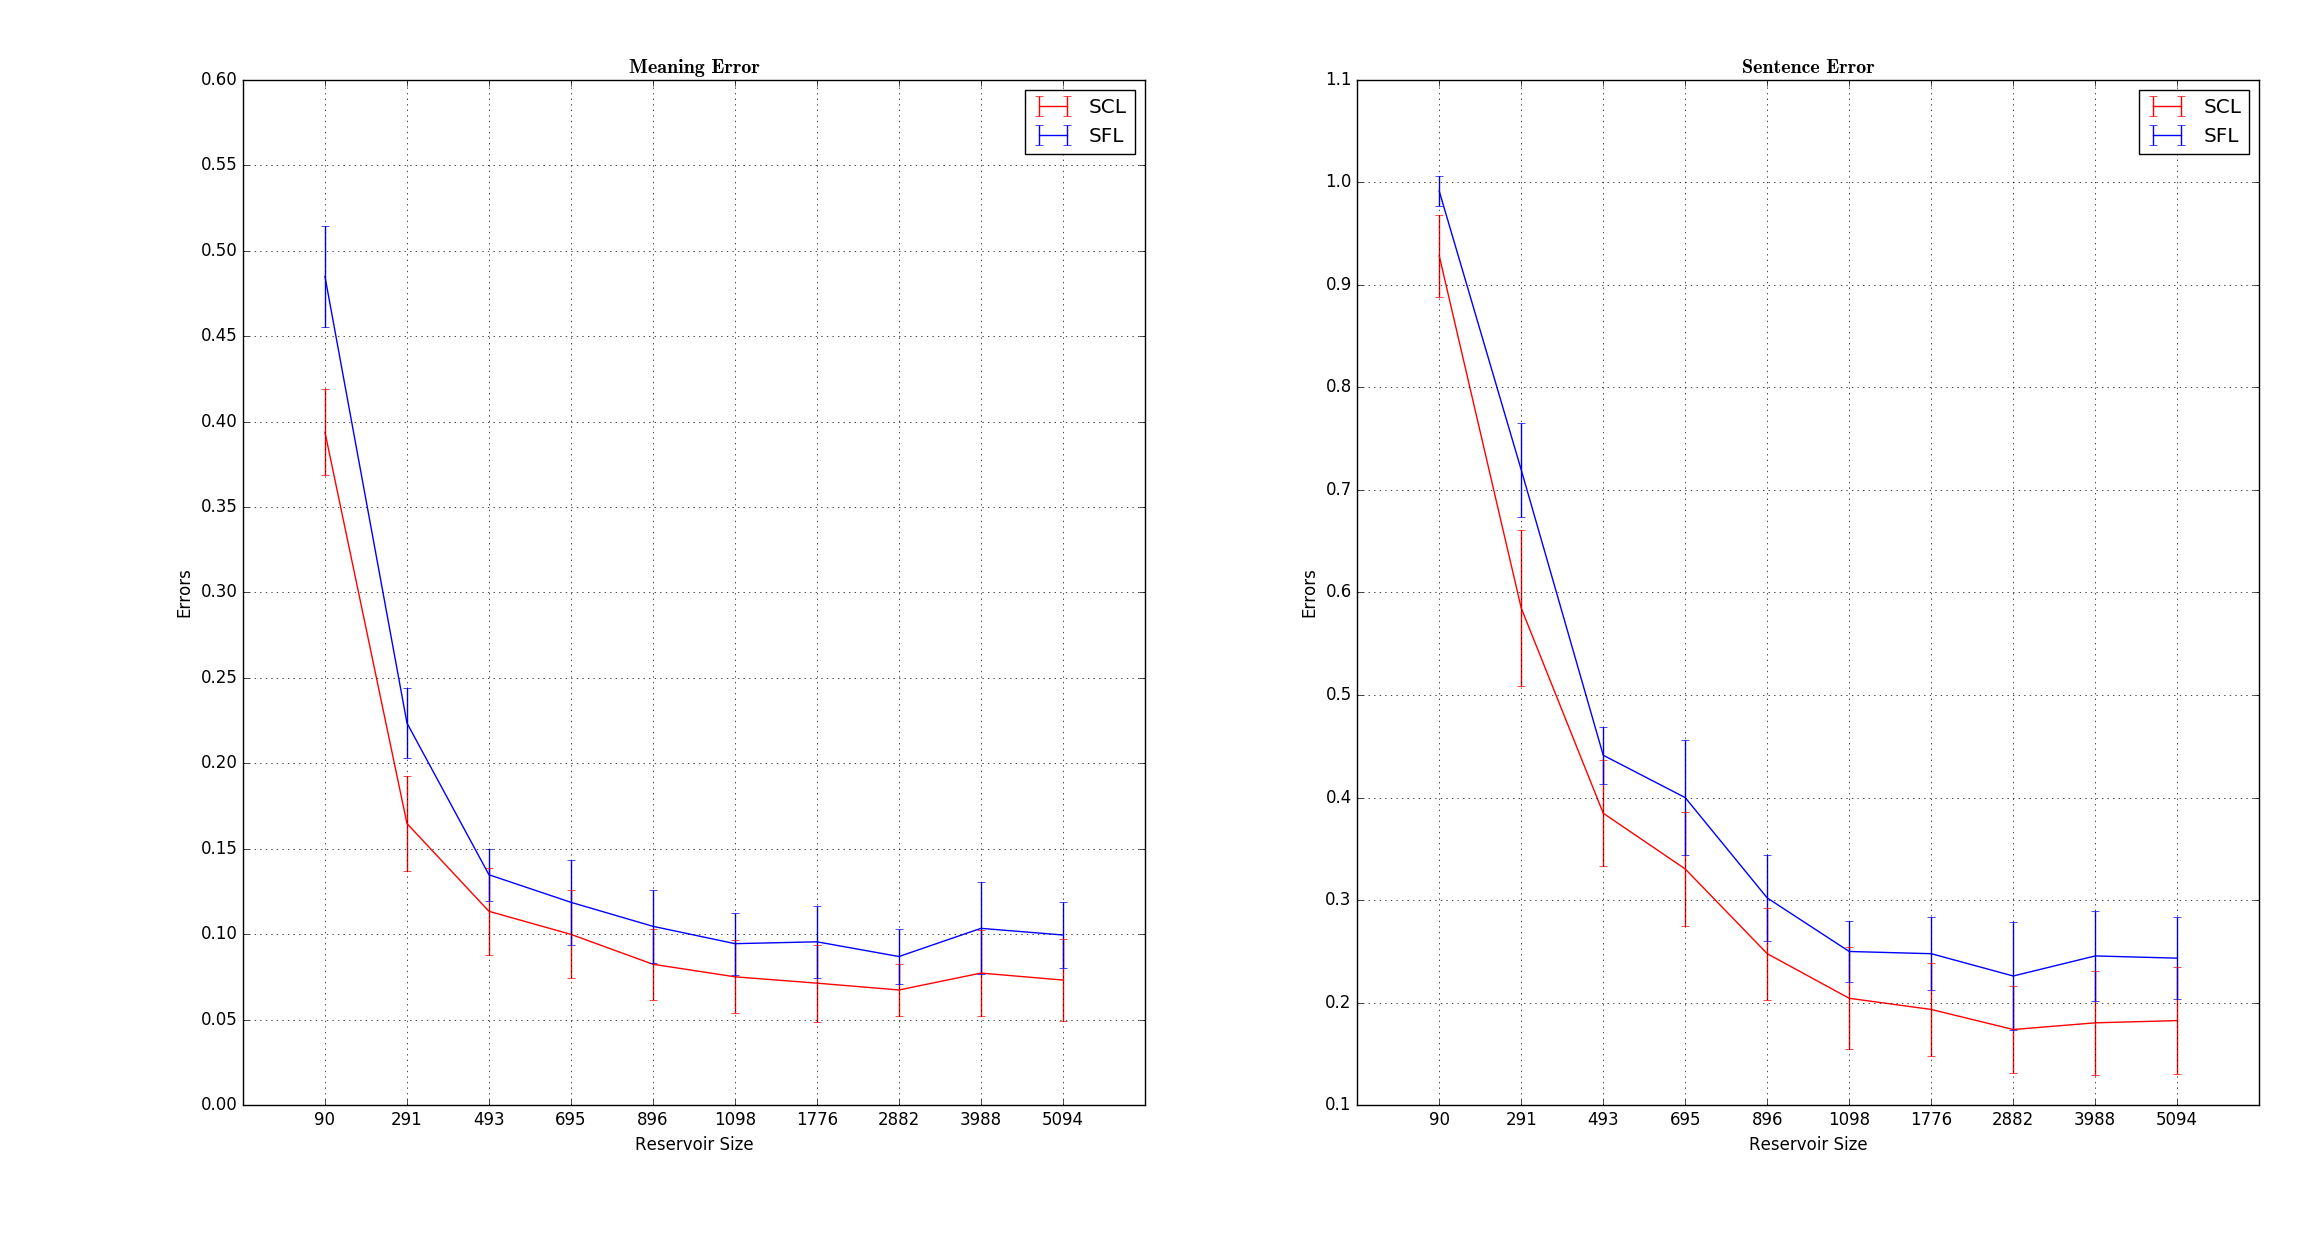
\includegraphics[width=1.0\linewidth]{reservoir_size_1}
\caption[Effect of reservoir size on Word2Vec-ESNM model]{\textbf{Effect of reservoir size on cross validation errors on Model Variant-1:} Description goes here.}
\label{fig:reservoir_size_1}
\end{figure}

\begin{figure}[hbtp]
\centering
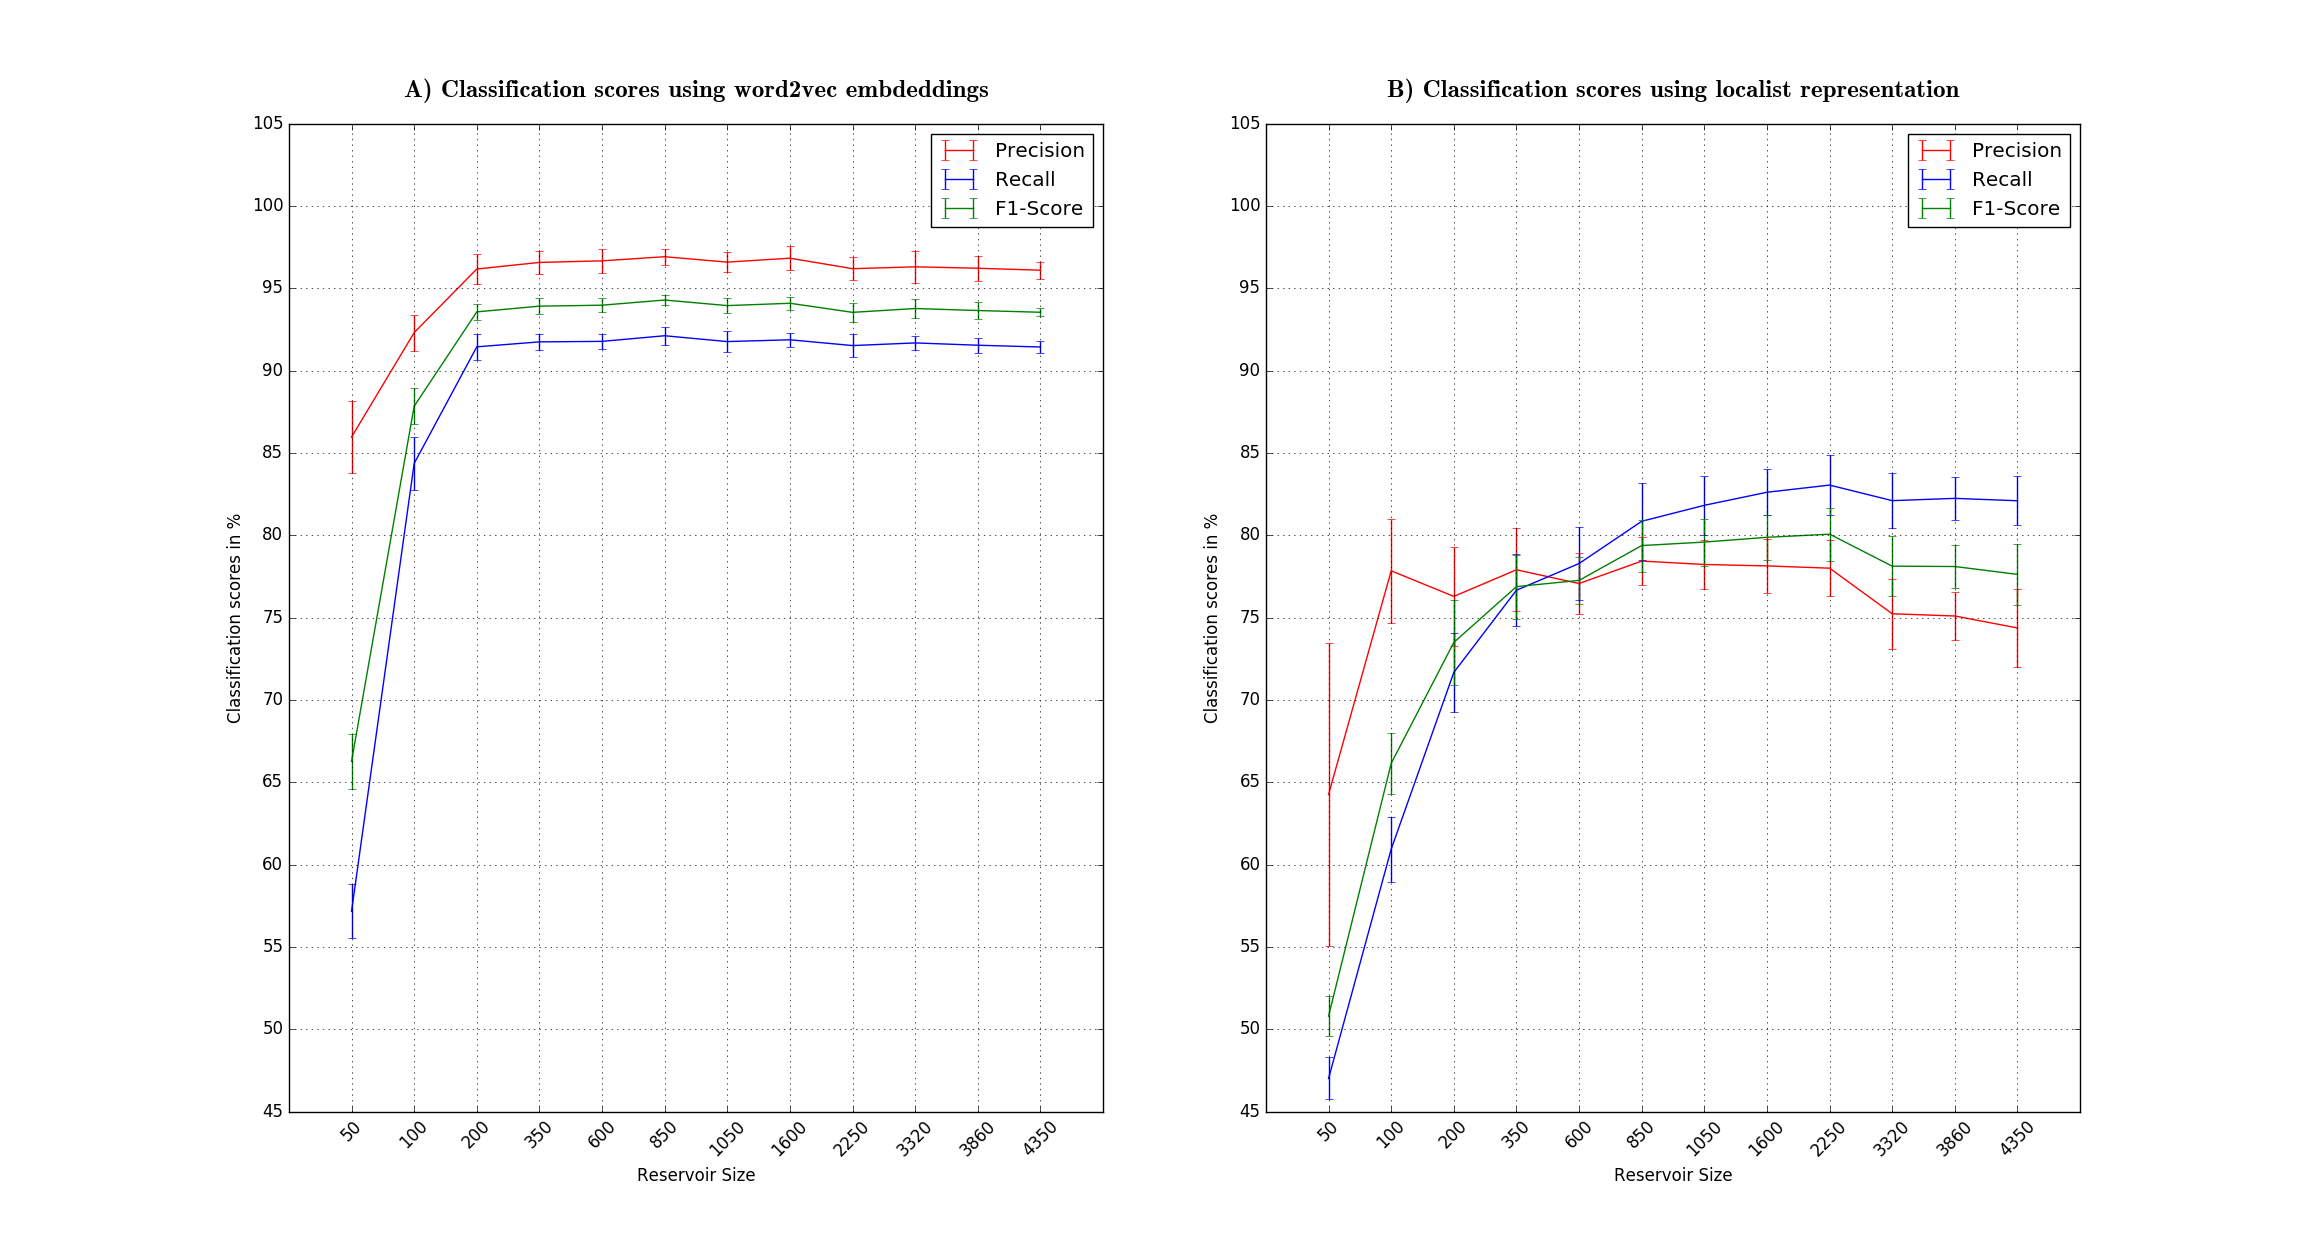
\includegraphics[width=1.0\linewidth]{reservoir_size_2}
\caption[Effect of reservoir size on Word2Vec-ESN model variant]{\textbf{Effect of reservoir size on classification scores of Model Varinat-2:} Description goes here.}
\label{fig:reservoir_size_2}
\end{figure}

\paragraph{Word2Vec-ESN model variant: } Figure \ref{fig:reservoir_size_2} shows the change in classification scores of model variant with increase in reservoir size. It can be observed that when using the word2vec vector (Configuration-1) the classification scores sharpely increases when the reservoir size is increased from 50 neurons to 250 neurons. As the reservoir size is further increased from 250 neurons, the classification scores remains stable with neglible drop. Whereas, in Configuration-2 (i.e. when using GF and Localist representation) the classification scores also improves, with increase in reservoir size from 50 to 250 neurons. As the reservoir size is further increased from 250 neurons, the recall is improved whereas the precision remains almost flat with neglibile improvement. As the F1-Score is harmonic mean of precision and recall, it was also slightly increased. Even the highest F1-Score of model variant observed at reservoir size 4500 in configuration-2, is much lower than that of obeserved at reservoir size 100 ($\approx 29 \%$ ) in configuration-1.

\subsection{Experiment-5: Effect of Corpus size}

Figure \ref{fig:corpus_size_1} shows the cross-validation errors rates with respect to corpus size on Word2Vec-ESN model. It can be observed that with increase in corpus size from $6 \%$  to $50 \%$, the meaning error sharply drops from some $12.18 \% (\pm 0.19 \%)$ to $2.96 \%(\pm 0.04\%)$ in SCL mode and from $11.96\%(\pm 0.35\%)$ to $4.17 \%(\pm 0.11\%)$ in SFL mode. Similarly, the sentence error also decreases from $54.84 \%(\pm 0.52\%)$ to $17.25 \%(\pm 0.39\%)$ in SCL and from $54.14 \%(\pm 1.28\%)$ to $22.41 \% (\pm 0.57\%)$ in SFL mode. When the sub-corpora size is $75\%$, where the model was trained only on $37.5\%$ of corpora size, the model already generalized with $2.72 \%(\pm 0.03\%)$ meaning error and $15.98 \% (\pm 0.30\%)$ sentence error in SCL mode and with $3.95 \%(\pm 0.11\%)$ meaning error and $21.33 \%(\pm 0.64\%)$ sentence error in SFL mode. 

However, it was also observed that, although the error rates gradually drops when the corpus size is further increased from $25\%$ to $100\%$ but the improvement rate of errors is very less. Thus further increase in corpus size won’t have much effect on cross validation error.

\begin{figure}[hbtp]
\centering
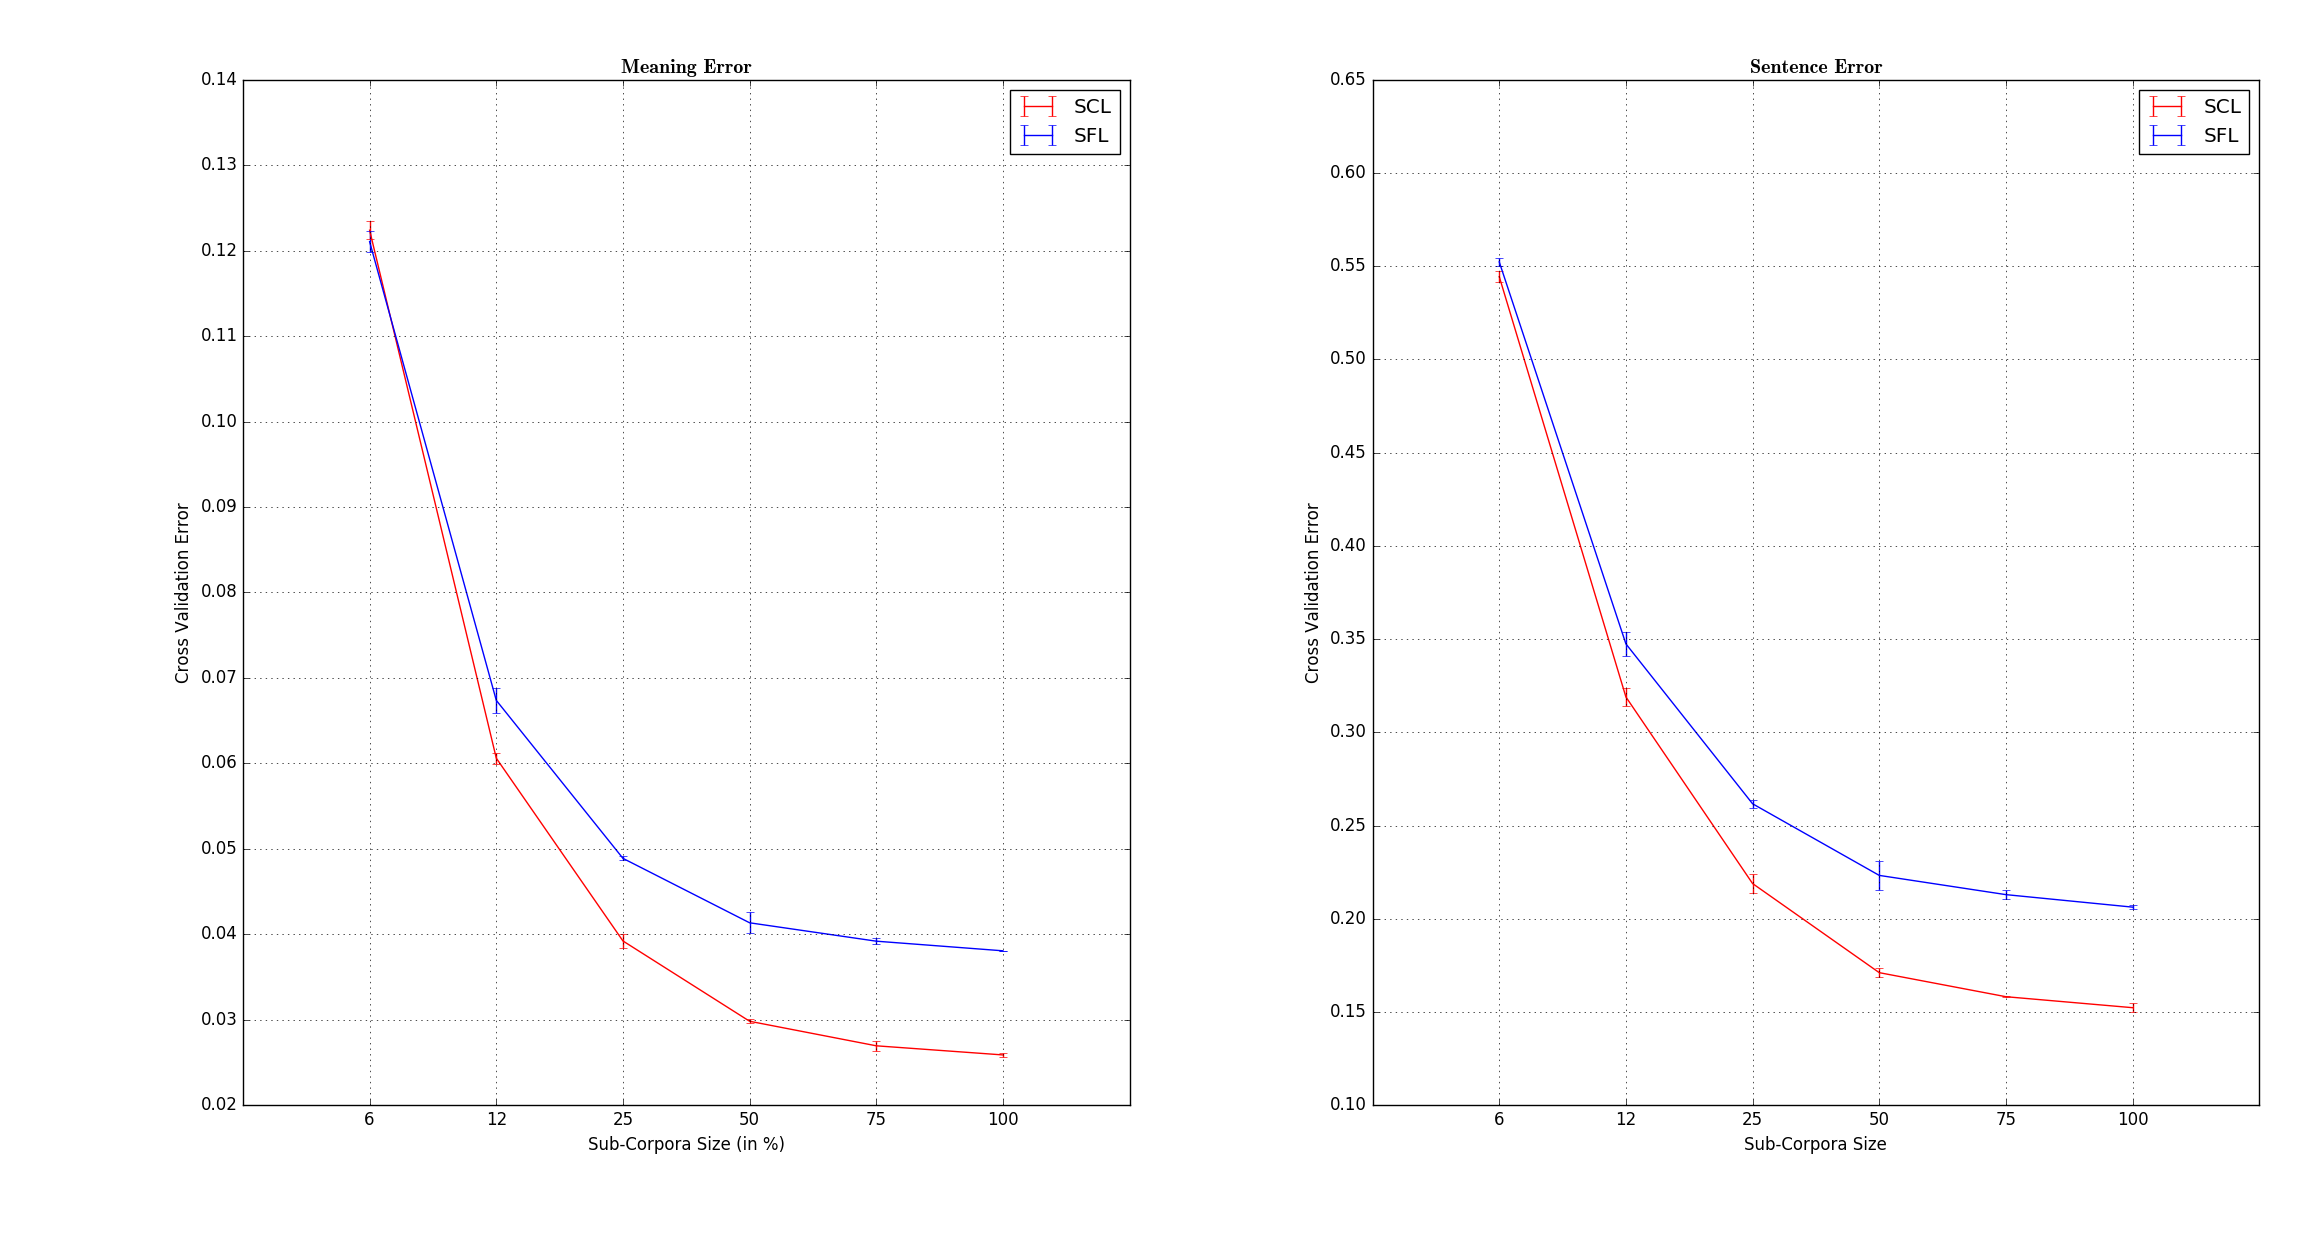
\includegraphics[width=1.0\linewidth]{corpus_size_1}
\caption[Effect of corpus size on Word2Vec-ESN model]{\textbf{Effect of corpus size on cross validation errors of Word2Vec-SN model in SCL and SFL mode.} }
\label{fig:corpus_size_1}
\end{figure}

\begin{figure}[hbtp]
\centering
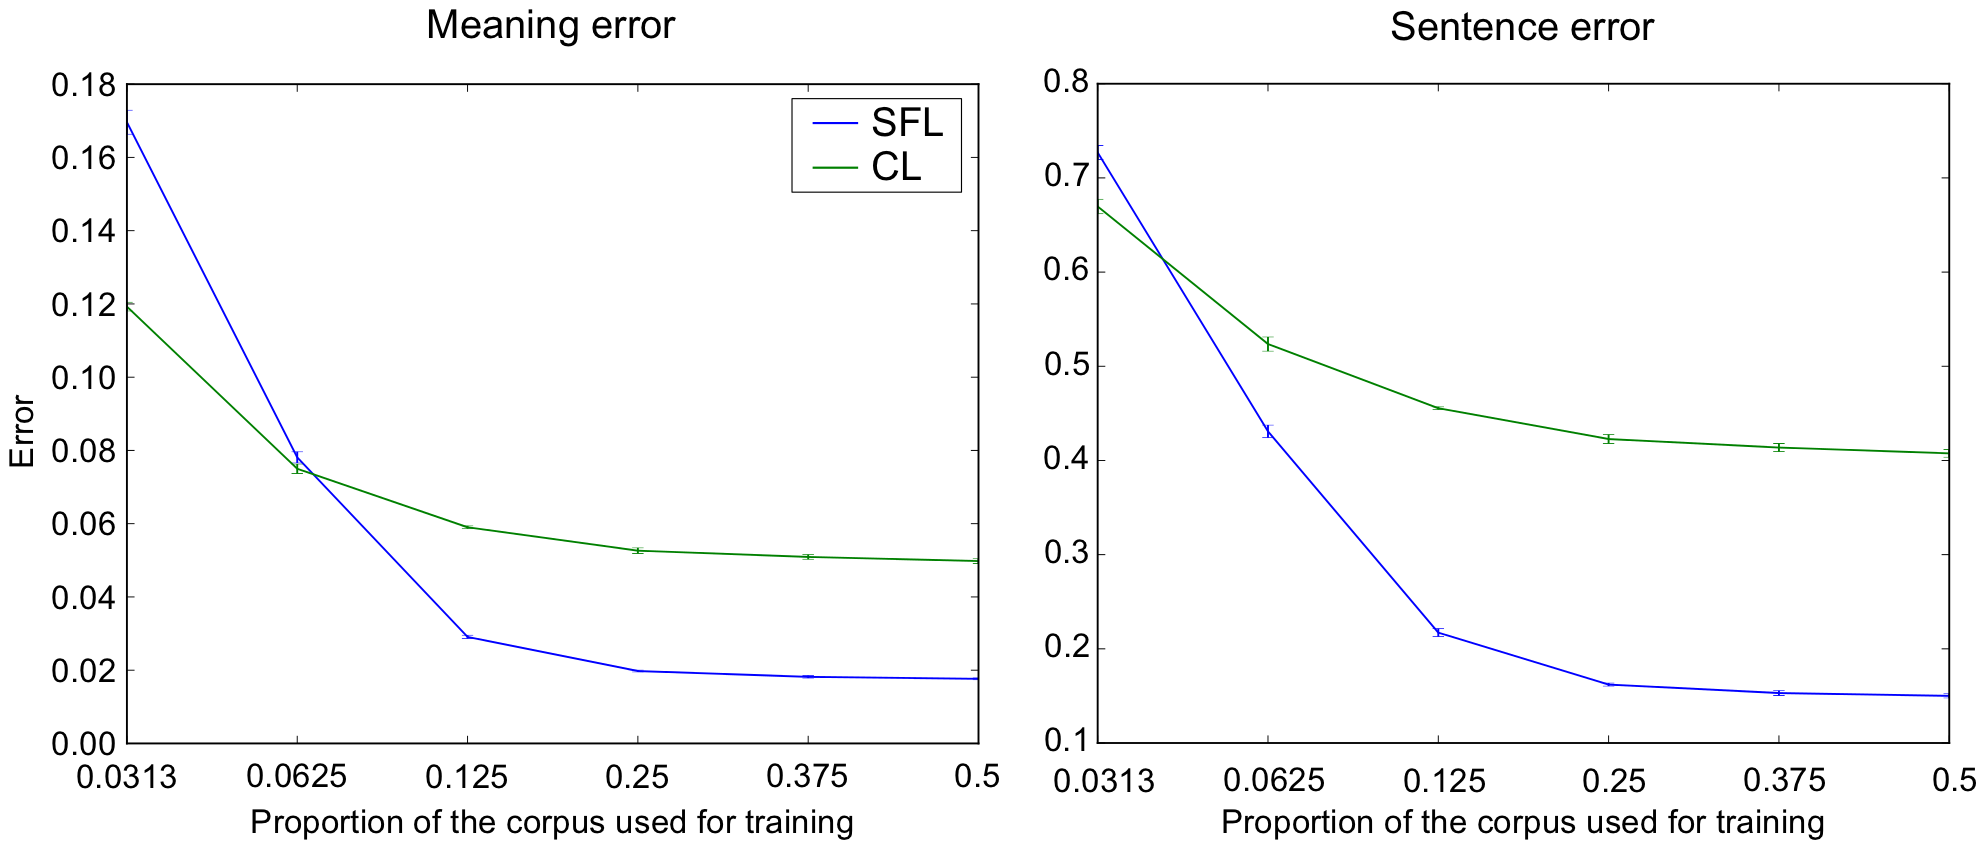
\includegraphics[width=1.0\linewidth]{corpus_size_xavier}
\caption[Effect of reservoir size on Word2Vec-ESN model variant]{\textbf{Effect of corpus size on cross validation errors using localist word vector as reported in [ref]:} Description goes here.}
\label{fig:corpus_size_xavier}
\end{figure}

Comparing the effect of corpus size on Word2Vec-ESN model with that of $\theta RARes$ model (see fig. \ref{fig:corpus_size_xavier}), it was observed that in SFL mode, with increase in corpus size from $6\%$ to $25\%$, the meaning error in $\theta RARes$ model dropped from $\approx 17\%$ to $\approx 4\%$ and sentence error dropped from $\approx 70\%$ to $\approx 20\%$, whereas in Word2Vec-ESN model meaning error dropped from $\approx 12\%$ to $\approx 5\%$  and sentence error dropped from $\approx 55\%$ to $\approx 26\%$. Also, with increase in corpus size further from $25 \%$ the cross-validation errors asymptotes in both the models with negligible improvement in error rates. Overall, the improvement in error rates with $\theta RARes$ model in SFL mode, is higher as compared to Word2Vec-ESN model.

Comparing the performance of both models in the SCL mode, the drop in meaning error almost remained equivalent with increase in corpus. Whereas, with increase in corpus size from $6\%$ to $100\%$, the sentence error in $\theta RARes$ model dropped from $\approx 65\%$ to $\approx 40\%$ and in Word2Vec-ESN model this drop was observed from $\approx 55\%$ to $\approx 15 \% $. 

\subsection{Experiment-6: Generalization on new corpus}

In the Table \ref{tab:corpus_373}, the sentence and best error values obtained with Word2Vec-ESN and $\theta RARes$ model are reported. The best error here represents the percentage of sentences whose meanings were predicted incorrectly in common within 10 model instances \cite{tra:xavier_hri}. The Word2Vec-ESN model with a reservoir of size 500 neurons, generalized with a sentence and best error of $42.65 \%$ and $26.54 \%$ respectively. Whereas with a reservoir of 1000 neurons, the Word2Vec-ESN model generalized with $40.29 \%$ and $25.73 \%$ sentence and best errors respectively. In comparision to $\theta RARes$ model, the mean sentence error in Word2Vec-ESN model improved by $26.31\%$ and $17.97\%$  with resevoir of size 500 and 1000 respectively. The best errors also improved by $17.96 \%$ and $9.12 \%$ with reservoir size 500 and 1000 respectively.

Although, the Word2Vec-ESN model generalized better with both the reservoir sizes (500 and 1000) as compared to $\theta RARes$ model, but the improvement in cross-validation error in Word2Vec-ESN model is comparatively less than $\theta RARes$ model. The mean sentence error and best error improved by $2.36 \%$ and $0.81\%$ respectively with increase in reservoir size in Word2Vec-ESN model. In $\theta RARes$ model, increasing reservoir size from 500 to 1000 leads to an improvement of $10.7\%$ mean sentence error and $9.65\%$ best error. 

\begin{table}
\centering
\begin{threeparttable}
\caption[Word2Vec-ESN model generalizing on new coprus]{Generalization error in SCL mode on corpus-373.}
\label{tab:corpus_373}
\rowcolors{2}{gray!25}{white}
\begin{tabular}{llll}
\toprule
Reservoir 	 		&  Error 	&  Word2Vec-ESN 			& $\theta RARes$ \\
\midrule                 
\textbf{500 N}	& mean(std.) 		& 42.65 ($\pm$ 1.36) 	& 68.96 ($\pm$ 2.03)  \\
					& Best 			& 26.54 					& 44.50  \\
\textbf{1000 N}	& mean(std.) 		& 40.29 ($\pm$ 1.13) 	& 58.26 ($\pm$ 1.37)\\
					& Best 			& 25.73 					& 34.85 \\
\bottomrule
\end{tabular}
\begin{tablenotes}
\small
\item 
Sentence and best errors (in $\%$) obtained with Word2Vec-ESN model and $\theta RARes$ in SCL mode with reservoir of size 500 and 1000 neurons. The results reported are mean and standard deviation of errors obtained from 10 reservoir instances. The best error here means the percentage of sentence errors common within all 10 reservoir instances \cite{tra:xavier_hri}. Simulation conditions for Wor2Vec-ESN model: Leave-one-out cross validation, SR=[] , IS=[] , LR=[]. 
\end{tablenotes}
\end{threeparttable}
\end{table}

\subsection{Experiment-7: Effect of Word2Vec word dimensions}

\paragraph{Word2Vec-ESN model: } Figure \ref{fig:word_dim_scl} and  \ref{fig:word_dim_sfl} represents the effect of word vector dimensions on cross-validation errors of Word2Vec-ESN model in SCL and SFL mode respectively. The corresponding errors are also reported in Table \ref{tab:word-vector-size}. In the figures we can see that from lower to upper limit of word vector dimensions studied, all the error measures in both the learning modes increased approximately by $2\%$. Also, the cross-validation errors remained almost equivalent with negligible fluctuations in the range 20 to 200 dimensions, with the mimimum errors obtained with word vectors of 30 dimensions ($ME= 14.23 (\pm 0.53), SE= 43.46 (\pm 0.70)$). When the word vector dimension is further increased to 300, we can see that all the error measures increased nearly by $2 \%$. Another interstin pattern which can be observed is that with all the word vector dimensions the model in SCL mode always performed better as compared to SFL mode. The similar relation between SCL and SFL model was also observed in previous experiments as well. Over we can say that the word vectors dimensions have negligible effect on the perofamance of Word2Vec-ESN model.

\begin{figure}[hbtp]
\centering
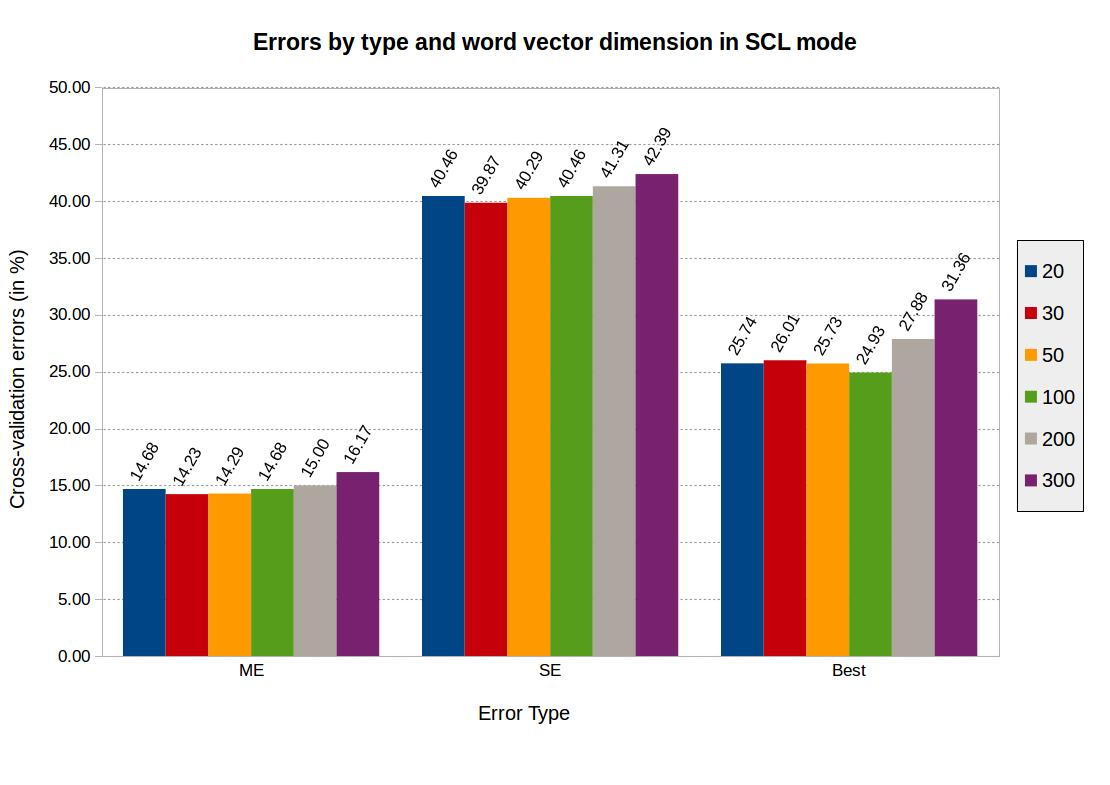
\includegraphics[width=0.9\linewidth]{word_dim_scl}
\caption[Effect of word vector dimensions on Word2Vec-ESN model]{Effect of word vector dimensions on cross validation errors of Word2Vec-ESN model in SCL mode.}
\label{fig:word_dim_scl}
\end{figure}

\begin{figure}[hbtp]
\centering
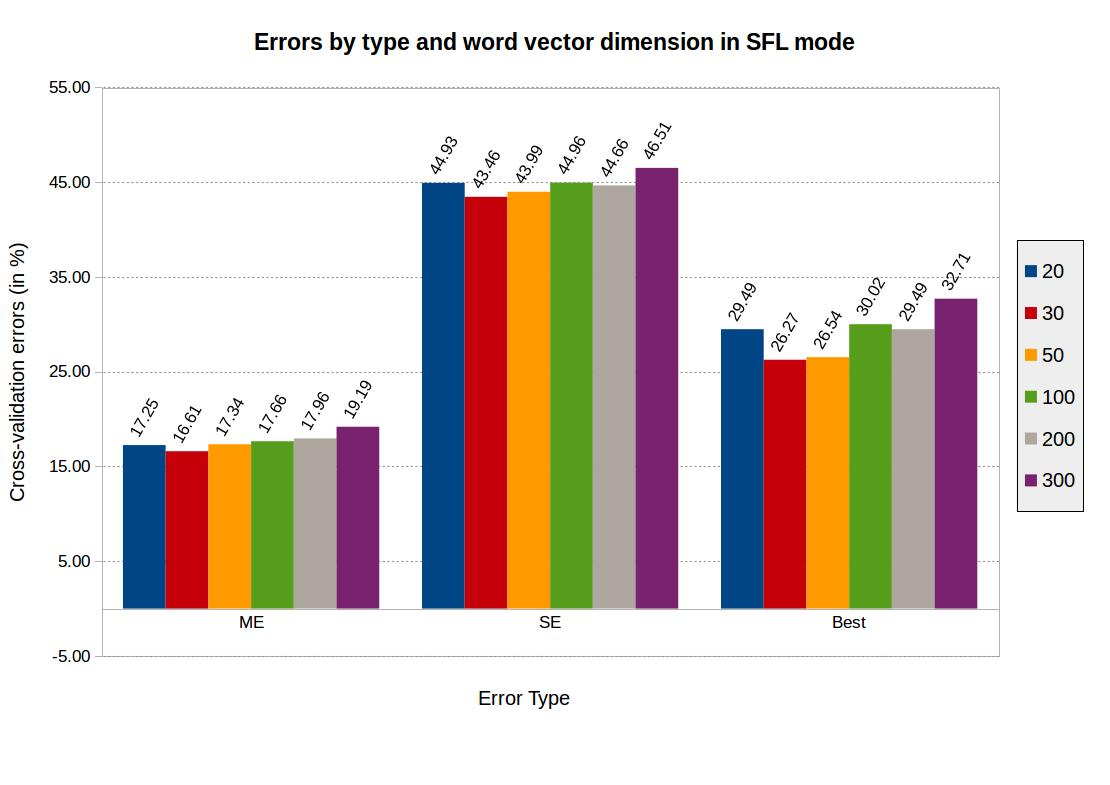
\includegraphics[width=0.9\linewidth]{word_dim_sfl}
\caption[Effect of word vector dimensions on Word2Vec-ESN model]{Effect of word vector dimensions on cross validation errors of Word2Vec-ESN model in SFL mode.}
\label{fig:word_dim_sfl}
\end{figure}


\subsection{Neural output activity of the Word2Vec-ESN model}

In the previous experiments, we observed that both the model variants generalized well and cross-validation error rates dropped with increase in corpus size. The 45 sentences of corpus-45 was added to corpus-462 to get the resultant corpus have 507 sentence (462 + 45). The readout activations of the Word2Vec-ESN model were then analysed for the input sentences to have the insight of how the system is learning the meaning. It was observed that the model is re-analyzing the thematic roles of input sentences across the time. The same behaviour was also observed by Hinaut et. al \cite{tra:xavier_hri, xavier:2013:RT} with $\theta RARes$ model.

Figure \ref{fig:act_analysis_1} shows the read out activations of second noun in following four sentences across time. Note that the sentences \ref{activation:sent-1} and \ref{activation:sent-2}  with active constructions whereas \ref{activation:sent-3} and \ref{activation:sent-4} are passive constructions.

\begin{enumerate}[noitemsep]
\item the man \textit{gave}(V1) the \textit{book}(N2) to the boy. \label{activation:sent-1}
\item the man \textit{took}(V1) the \textit{ball}(N2) that \textit{hit}(V2) the glass. \label{activation:sent-2}
\item the boy \textit{caught}(V1) the \textit{ball}(N2) that was \textit{thrown}(V2) by the man.  \label{activation:sent-3} 
\item the ball was \textit{pushed}(V1) by the \textit{man}(N2).  \label{activation:sent-4}
\end{enumerate}

Each coloured lines in the graph represents the possible thematic roles of Noun-2 (N2), which can have one of the three possible roles i.e. agent (A), object (O) or recipient(R) with resepct to either Verb-1 (V1) or Verb-2 (V2).N2 is marked in red and verbs are marked in green. In the figure the role `N2-A-V1' can be interpreted as noun-2 is the agent of verb-1.

As all the four sentences start with `the', activations at this word is same for all four sentences. With the introduction of the first noun (`man') in sentences \ref{activation:sent-1} and \ref{activation:sent-2}, the readout activations of role N2 as object of V1 (N2-)-V1) goes above the threshold 0 and thus the model predicts that the N2 (`book') is the object of V1 (`gave'). In sentence \ref{activation:sent-3}, with the arrival of first noun (`boy') a competition between roles N2-A-V1, N2-A-V2 and N2-O-V2 can be seen, but only the role N2 as Agent of V1 (`pushed') making it above the threshold. Whereas,in sentence \ref{activation:sent-4}, the activation of role with N2-A-V1 is higher when the first noun (`ball') is encountered, but with the arrival `was' the role of N2 is changed as recipient of V1 (`pushed').

With the arrival of the V1 (`took'), in sentence \ref{activation:sent-2}, the activation for N2 as an agent of V2 goes above threshold indicating the presence of V2 (`hit') in the sentence even before the model has encountered the second verb. Whereas in sentence \ref{activation:sent-1} the activation of role N2 as agent of V1 maintained and no other roles managed to cross the threshold with the arrival of V1 (`gave'). In sentence \ref{activation:sent-3} and \ref{activation:sent-4}, with the arrival of V1 (`caught' and `pushed') one can notice the re-analysis made by the model, with activation of N2 as agent of V1 going below threshold and taking the new role as object of V1 (`gave') in sentence \ref{activation:sent-3}. Also, in sentence \ref{activation:sent-3}, the activation of role N2 as object of V2 (N2-O-V2) goes above threshold whereas in sentence \ref{activation:sent-4} the previously predicted role N2-R-V1 goes below threshold with the arrival of V1 (`pushed').

Throughout the rest of sentence \ref{activation:sent-1}, the prediction N2-O-V1 is maintained with some minor ups and downs. In sentence \ref{activation:sent-2}, the predictions of N2 alternates between O-V1 and A-V2. While the arrival of "the" and "ball" seems to favour O-V1, arrival of "that" changes the prediction again to A-V2. In both cases, the activation of both the role 0-V1 and O-A2 remains above threshold. In sentence \ref{activation:sent-3} the model sees both O-V1 and R-V1 as the prefered predictions, both being almost on the same level and only alternating slightly . In sentence \ref{activation:sent-4}, the prediction of role N2 as agent of V1 do not change again throughout the sentence ever since arrival of V1 (`pushed').

\begin{figure}[hbtp]
\centering
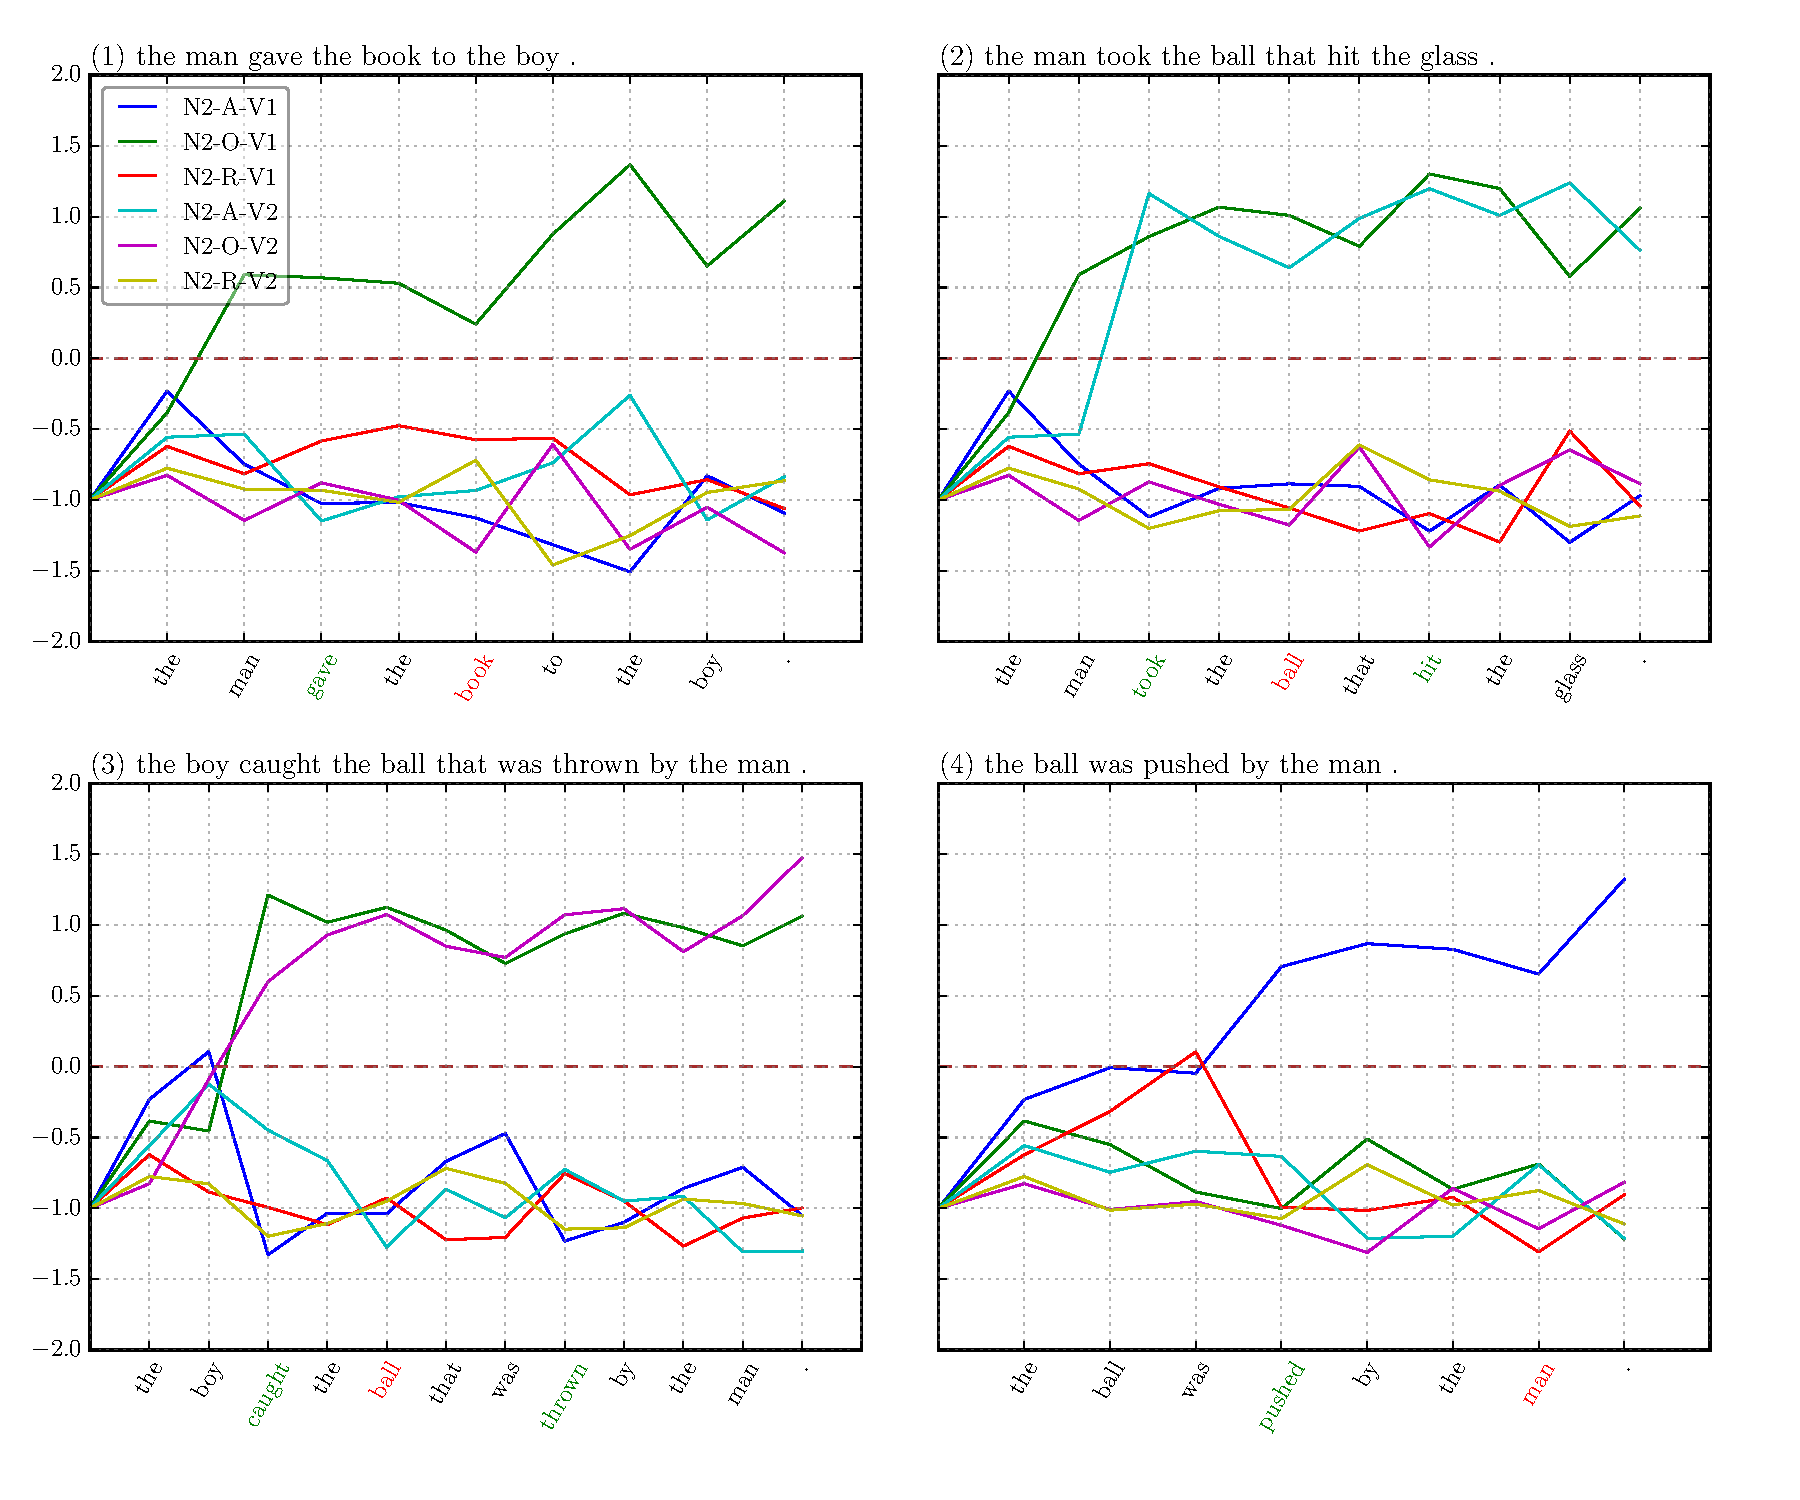
\includegraphics[width=1.0\linewidth]{act_analysis_1}
\caption[Online re-analysis of activation by Word2Vec-ESN Language model:]{\textbf{Short discourse processing by Word2Vec-ESCN Language model:} Each coloured line shows the thematic role of Noun-1 (tick marked in red) with respect to Verb-1 and Verb-2 (ticks shown in green). The coded meaning for the second segement of sentence is resolved using the information from first segment of sentence. Thus, also resolving the anaphoric reference to `he' and `it'. Model predictions: A) N1 is agent of verb-1 and verb-2. B) N1 is agent of object of verb-1 and verb-2. C) N1 is agent of verb-1 and object of verb-2. D) N1 is object of verb-1 and agent of verb-2.}
\label{fig:act_analysis_1}
\end{figure}

\begin{figure}[hbtp]
\centering
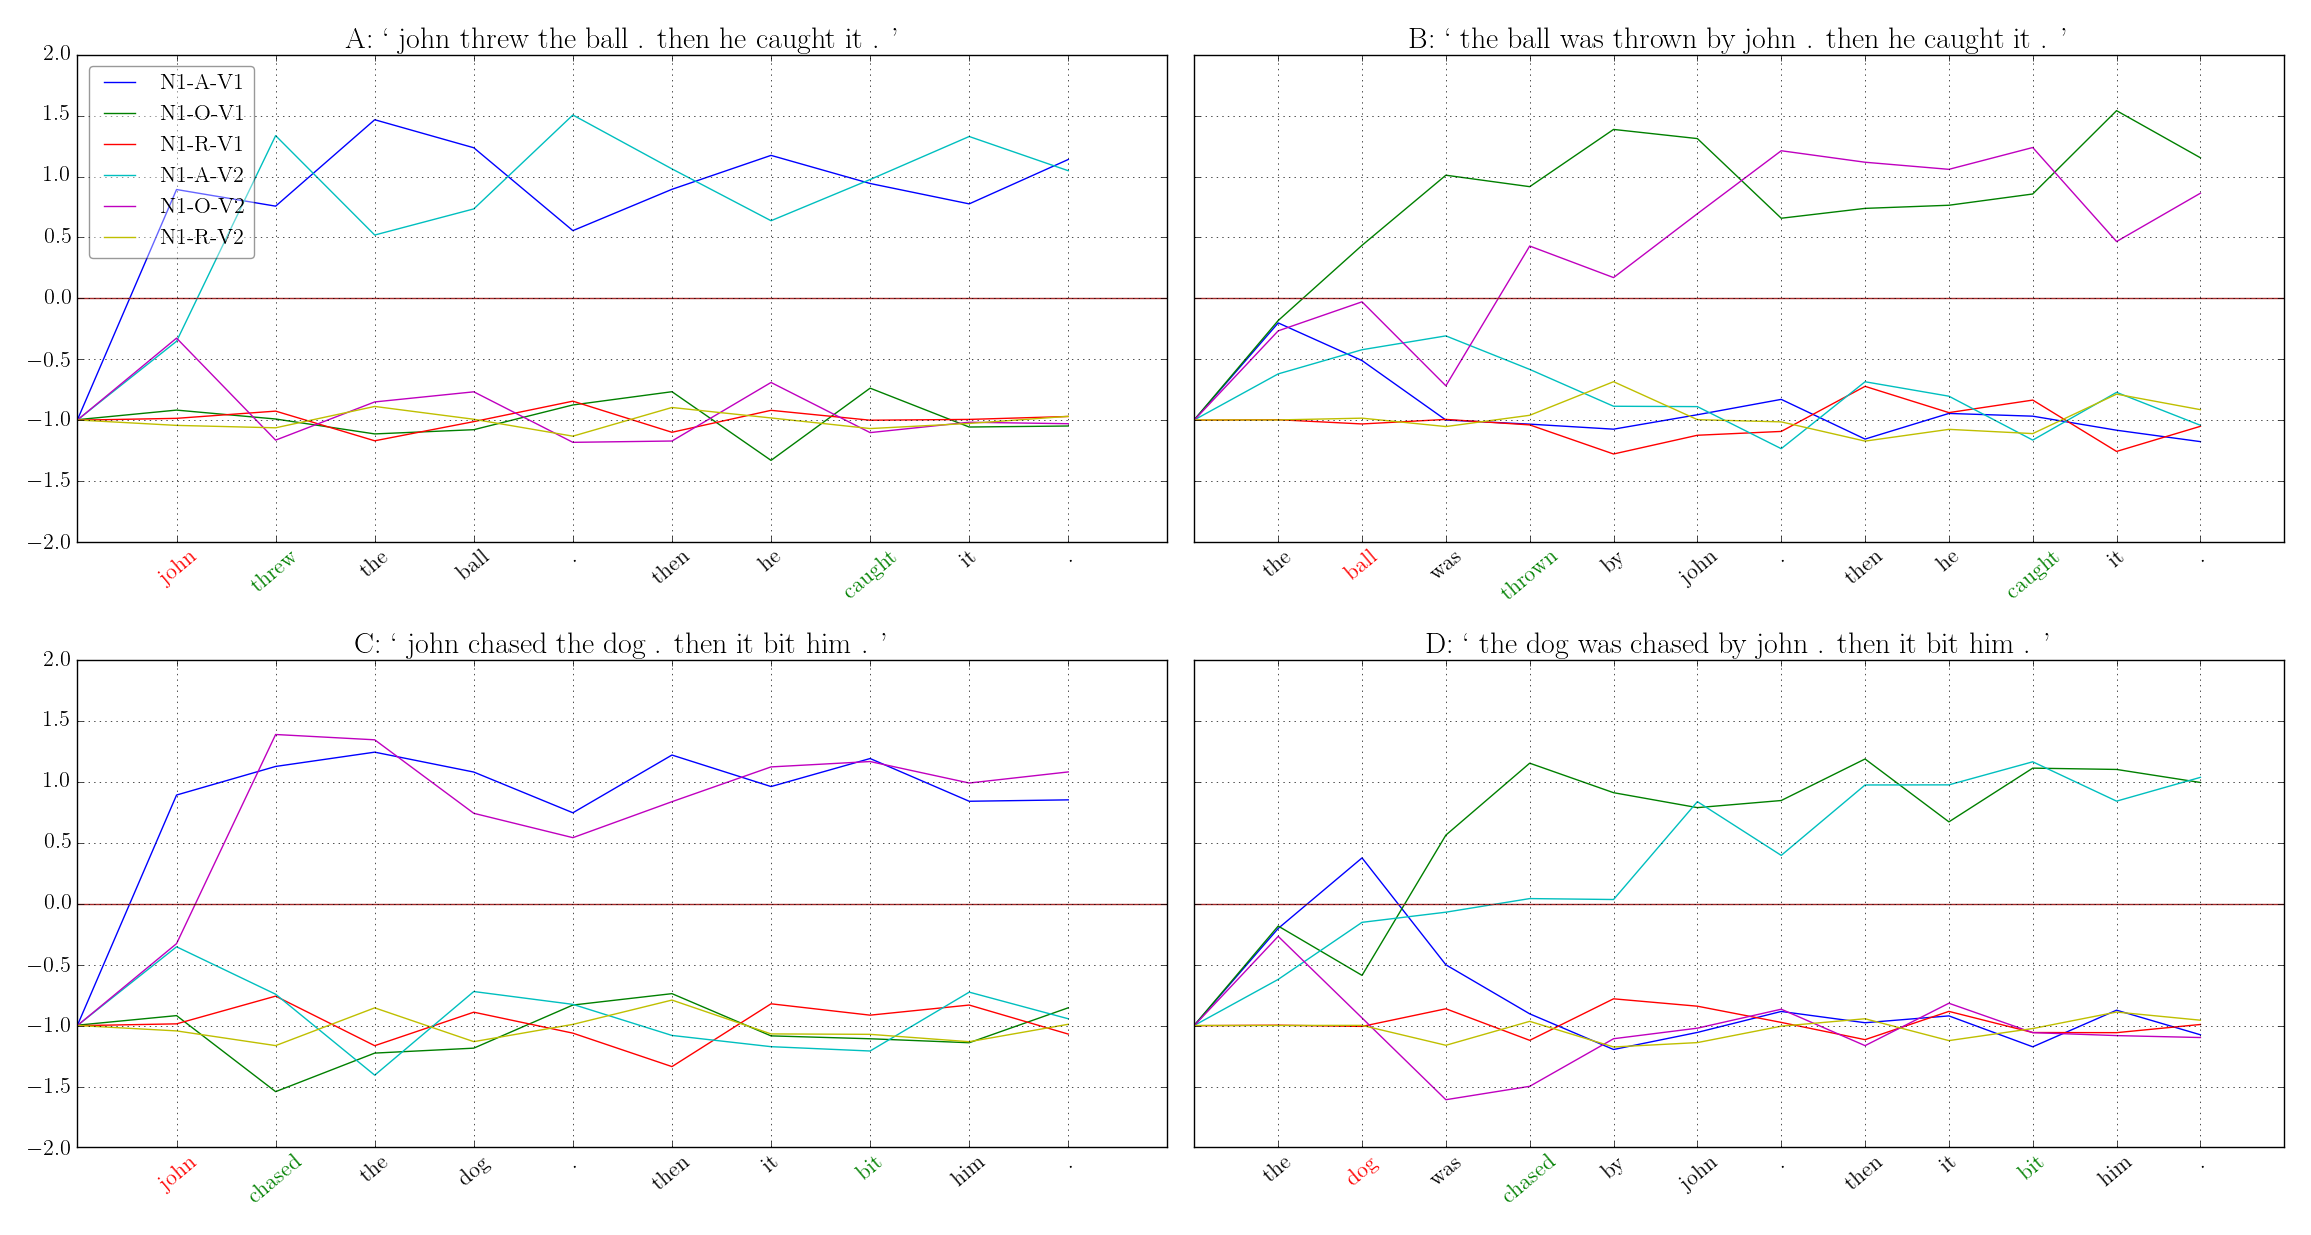
\includegraphics[width=1.0\linewidth]{act_analysis_3}
\caption{\textbf{Effect of corpus size on cross validation errors using localist word vector as reported in :} Description goes here.}
\label{fig:act_analysis_3}
\end{figure}

\paragraph{Discourse processing: } Figure \ref{fig:act_analysis_3} shows the read out activations of Noun (N1) in the following sentences with two-sentence discourse segment across time. 

\begin{enumerate}[noitemsep,label=(\Alph*) ]
\item \textit{John}(N1) \textit{threw}(V1) the ball. Then he \textit{caught}(V2) it. \label{activation:sent-a}
\item The \textit{ball}(N1) was \textit{thrown}(V1) by John. Then he \textit{caught}(V2) it. \label{activation:sent-b}
\item \textit{John}(N1) chased the dog. Then it \textit{bit}(V2) him.\label{activation:sent-c}
\item The \textit{dog}(N1) was \textit{chased}(V1) by John. Then it \textit{bit}(V2) him.\label{activation:sent-d}
\end{enumerate}

Note that the first segment of sentences \ref{activation:sent-a} and \ref{activation:sent-c}, \ref{activation:sent-b} and \ref{activation:sent-d} have the same grammatical form, whereas the second part of the senteces \ref{activation:sent-a} and \ref{activation:sent-b}, \ref{activation:sent-c} and \ref{activation:sent-d} have the same grammatical structure.

One can see in the figure \ref{fig:act_analysis_3} that the model was able to resolve the roles for second verb (V2) present in second segment of all the sentences, using the information from first part of the sentences, although there were no explicit nouns in the second segment of sentence. Thus also the anaphoric reference to `he' and `it' is also resolved.

Comparing sentences \ref{activation:sent-a} and \ref{activation:sent-b}, both have the same second segment i.e. ``then he caught it", but model predicted different coded meaning for both this segment of sentence, depending on the first segment of sentence. In \ref{activation:sent-a} the model makes an eary prediction that N1 is the agent of the second verb (`caught'), whereas in sentence \ref{activation:sent-b}, N1 is predicted as the object of the second verb. Similarly, the senteces \ref{activation:sent-c} and \ref{activation:sent-d}, the second segment is same in both the sentences i.e. `` the it bit him", but the model predicted the N1 is object of V2 (`bit') in sentence \ref{activation:sent-c} and N1 is agent of the same second verb.


Also, notice that the roles for N1 with respect to V2, is predicted earlier in sentences \ref{activation:sent-a} and \ref{activation:sent-d} as comared to that of sentence \ref{activation:sent-b} and \ref{activation:sent-d}, where in the latter the  presence of V2 and the role of N1 with respect to V2 is confirmed only after the arrival of V1. With the arrival of `was' and V1 (`chased') in sentence \ref{activation:sent-d}, the model changes its previous prediction that N1 is agent of V1 and assigns a new role that N1 is object of V2 (`bit').  





















